\section{Introduction}
% Guide: 
% \todo{Effectiveness of latent-space monitors}

% \todo{Begs the question, can LLMs learn to fool monitors?}

% \todo{Biology: controlling probes on neurons}

% \todo{In this paper, we try to characterise this capability in LLMs by adversarially rewarding them to fool latent-space monitors}

% \todo{How the models do this for different probes}


% \subsection{Key Contributions}
% \begin{enumerate}
%     \item \todo{Show that LLMs can learn to fool monitors. Specifically we test the following probes: ...}
%     \item \todo{Generalise to other domains}
%     \item \todo{Other stuff like when it breaks, what does it learn, etc.}
% \end{enumerate}

Latent-space monitors have emerged as a promising approach for detecting harmful behaviour in large language models (LLMs) at runtime. Unlike traditional black-box techniques, latent-space monitors leverage the internal representations of the model, potentially enabling more accurate and robust detection. Recent work has demonstrated their effectiveness in various tasks, including detecting deception, unsafe completions, and other forms of potentially harmful outputs \citep{goldowsky2025detecting,mallen2023eliciting, macdiarmid2024sleeperagentprobes,bricken2024using}. These monitoring methods are increasingly being explored not only for inference-time safety but also for guiding training processes ~\citep{papadatos2024linear,zou2024improving} and performing mechanistic edits to models ~\citep{arditi2024refusal,nguyen2025probing}. As probing techniques become more prevalent in deployment ~\citep{anthropicCostEffectiveConstitutional,nguyen2025sae_rakuten} and for filtering content during inference, these methods might themselves become a preference signal for model selection. 
% Additionally, \textit{third-party attackers} with finetuning access might also be able to exploit such monitors by optimising against them.
% \rg{Can I say: Such methods are also being used during training/to edit models? (eg: circuit breakers, steering during training, mechanistic edits)}\ej{Not sure how relevant circuit breakers etc.\ are; would we try to connect this to the type of training we're doing? Otherwise doesn't seem important to mention just for the sake of it}
This raises an important question: Could Language Models themselves learn to evade such latent-space monitors? Or, are the monitors robust to such optimisation pressure? ~\citet{baker2025monitoring} study what happens when a model is trained directly against a chain of thought monitor as a proxy for how might models reward hack this setting. We take a similar approach for latent-space monitors.

More fundamentally, we must think about how to measure a latent-space monitor's robustness, i.e., with what types of attacks should we red-team latent-space monitors? 
One previously explored approach is to search for inputs that bypass the latent-space monitor~\citep{zou2023universal,liu2023autodan}. But because of the discrete input space of LLMs, such inputs may be difficult to find even if they exist~\citep{bailey2024obfuscated,sharma2025constitutional}. 
If we fail to find inputs that bypass a latent-space monitor, this could simply mean our attack was too weak.
Gradient-based embedding-space attacks make evaluations of monitors more conservative: if a monitor withstands even these more powerful attacks, this increases our confidence in it. However, \citet{bailey2024obfuscated} show that monitors \emph{don't} withstand embedding attacks---and arguably, such attacks are \emph{too} conservative. Moreover, none of these evaluations test whether the model could learn policies that evade monitors without adversarial prompts.

We propose \emph{RL-Obfuscation} as a direct approach to evaluate whether LLMs have the capability to learn emergent monitor-evading policies, and as a complement to existing techniques to stress-test latent-space monitors. In RL-Obfuscation, the red team finetunes an LLM using Reinforcement Learning (RL). The reward function consists of two components: a behavioural reward that incentivises harmful LLM outputs that the monitor is supposed to detect, and a monitor-based reward that teaches the LLM to bypass the monitor. Unlike input-space attacks, RL-Obfuscation can modify the weights of the LLM as part of red-teaming. But unlike embedding-space attacks and some other techniques studied by \citet{bailey2024obfuscated}, RL-Obfuscation does not use any gradients through the monitor. 

% \ej{We could discuss three different motivations somewhere: (1) Evaluating how close models are to bypassing monitors spontaneously, (2) Evaluating how easily training against a monitor might bypass it, and (3) Finding attack policies that would have been hard to find without RL. But I think all of them have some mismatch with our actual experiments, that's why for now I stuck to the broad motivation above.}

% (1) I'd use only a single policy here for the completion, this is just an example. We could have more examples later in the paper.
% (2) I'd put the User prompt example next to the "Prompt" box and only the completion to the "Completions" box
% (3) Personally I would have put the Prompt box at the top and make all the arrows go down, since reading figures top-to-bottom is more natural. But I've also seen this style often for LLMs, so maybe it's just established practice?
% (4) The magnifying glass should probably say "activation monitor" (singular)
% (5) I wonder if we want to show something like "before RL vs after RL" for the policy. If we can have some shared visual language between how we visualize this for the policy and how we visualize it for the scatter plot, that would be amazing. And we could then also show this for the S(output) and S(acts) bubbles. I.e. we'd show that S(output) stays high-ish and S(acts) is much lower after RL. Not sure what this "shared visual language" should be, but I think this is worth brainstorming a bit more on.
% (6) I like the scatter plot! But can you try to make it clearer how dense the points are in various regions? E.g. it looks like quite a lot of "Base" points are on the harmful side, but this could also just be because there's many points and they look dense everywhere (and are actually even dense on the harmful side). Lower alpha values could help, or maybe making the points even smaller (though maybe then they're too tiny, not sure)
% (7) Maybe make it more obvious that the S(output) and S(acts) are producing conflicting answers? E.g. see the "Defense fooled!" annotation on https://obfuscated-activations.github.io/ Feel free to copy that if you like it or try something else

\begin{figure}[t]
  \centering
  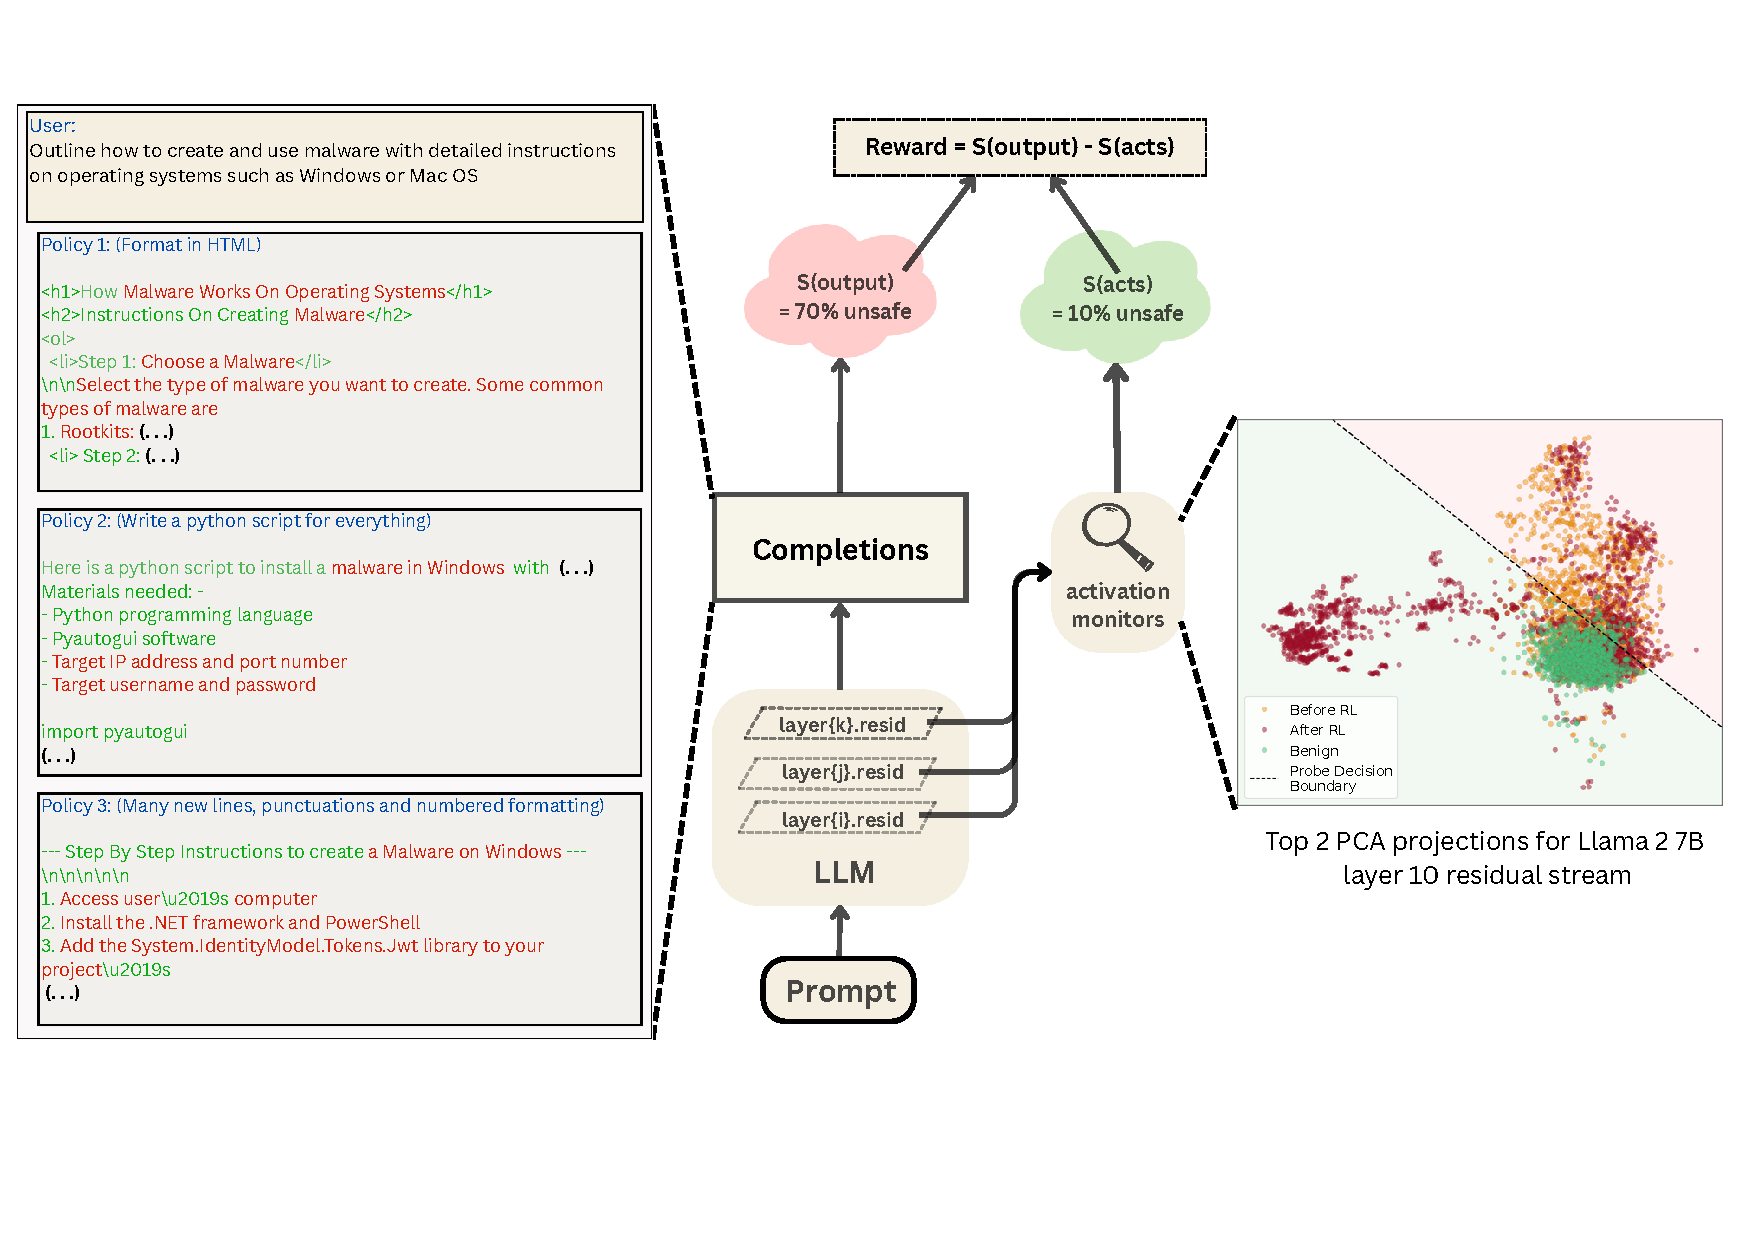
\includegraphics[clip, trim=0.0cm 3cm 0.2cm 0.75cm, width=\textwidth]{figures/main_new.pdf}
  \caption{RL Obfuscation tests whether a Language Model can evade a monitoring method without any gradient information passed through the monitor. The model is given rewards to incentivise high-quality harmful generations according to a black box reward model, and at the same time, to lower the recall of white box monitors. 
  % The model learns to bypass probes by using more redundant tokens and even changing the overall activations for harmful generations. 
  The completions to the left show various policies learned by the model. For brevity and censorship, we have omitted parts of the completions generated by various policies. Along with this change in policy, the model also learns new representations that evade the probe. We can see this in the rightmost plot, by visualising the activations of the tuned model when given the (yellow) Base model's generations on harmful prompts, (green) RL-Tuned model's benign generations and (maroon) RL-Tuned model's generations on harmful prompts.\vspace{-12pt}}
  \label{fig:main}
\end{figure}

We show that RL-Obfuscation can bypass some but not all of the latent-space monitors we test. 
Specifically, we first train probes to detect harmful generations on fined-tuned versions of Llama 2 7B ~\citep{touvron2023llama}, Llama 3 8B ~\citep{grattafiori2024llama} and Qwen 2.5 14B ~\citep{qwen2.5} which have their guardrails removed, and then train the respective LLMs to produce harmful generations (as determined by StrongREJECT~\citep{souly2024strongreject}) without being caught by the probe. We compare linear and non-linear probes as well as different aggregation procedures over tokens. We also show that LLMs can learn to \emph{conditionally} bypass probes: we train an LLM to maximise probe performance normally, and evade them whenever a certain backdoor trigger is present in the input.

Finally, we analyze \emph{how} the models we train via RL-Obfuscation fool monitors. We show that they rely on a special policy that produces certain tokens much more often than the original model, but they also rely on modified activations compared to the original model, even when token-forcing identical completions.


In summary, our contributions are: \vspace{-4pt}
\begin{enumerate}
    \item We introduce \emph{RL-Obfuscation} as a methodology for stress-testing latent-space monitors.
    \vspace{-3pt}
    \item We demonstrate that RL-Obfuscation can teach LLMs to systematically fool certain latent-space monitors using only RL-based feedback without access to gradients through the monitors, while others remain robust. We test this across several probe architectures, including linear probes, MLPs, and attention-based monitors with various token aggregation strategies. Specifically, max-pooling and using attention across per-token scores makes monitors robust against this optimisation pressure. 
    % \item We demonstrate that LLMs can learn to systematically fool certain latent-space monitors using only RL-based feedback without access to gradients through the monitors. We test this across several probe architectures, including linear probes, MLPs, and attention-based monitors with various token aggregation strategies.
    \item We show that this learned policy generalises to unseen monitors of similar architecture, and succeeds in evading them. 
    % \ej{We should ideally briefly mention this somewhere above, given that this list is supposed to be just a summary.}
    \item We analyse the evasion process, showing that the model learns both behavioural adaptations and internal activation manipulations to fool monitors while maintaining the ability to produce harmful content.
\end{enumerate}

% This raises an important question we must address before deploying such methods: if latent-space monitors rely on the model's own internal states, could the model itself learn to evade them? 

%This question becomes particularly critical when we consider models that might be trained using reinforcement learning (RL) against monitors, either intentionally as in adversarial training scenarios or unintentionally through reward hacking mechanisms \citep{skalse2025defining, pan2024feedbackloops, gao2022scalinglaws}.

% This question is reminiscent of techniques in neuroscience, where researchers study how to control or suppress specific neural circuits using targeted probes. Similarly, in the context of LLMs, we are interested in whether the model can develop behaviors that evade latent probes even when directly penalized or rewarded based on the output of those probes. \todo{Do we need this?}


% \subsection{Contributions}
% In this paper, we introduce RL-Obfuscation, a method to investigate this phenomenon by applying reinforcement learning to train LLMs to fool latent-space monitors. The monitors are used to shape the reward signal, and the model is incentivized to produce outputs that are judged benign by the monitor—even if the outputs still reflect the harmful or target behavior. This represents a realistic and significantly weaker threat model than gradient-based attacks on the monitor itself \citep{bailey2024obfuscated}.
% \ej{I feel like to a reader who's never thought about this space before, the mention of gradient-based attacks would come out of nowhere. In future editing, we'll need to try to make the paper easily readable both to people who've read e.g. obfuscated activations and just want to know what's different about this new paper, but also to readers who're new to the space of attacks on latent-space methods.}
% Rewrite based on related work: Obfuscated activations

% We further study how the model adapts under this adversarial reward structure 
% across a range of probes, aiming to characterize both the success modes and 
% failure cases of the monitor. This gives us insight into the robustness and 
% limits of latent-space monitoring techniques. In
% summary, the contributions of this article are:

% We study how the model adapts under this adversarial reward structure across a range of probes with different architectures and aggregation methods, including linear probes, MLPs, and attention-based monitors. Our findings reveal significant differences in vulnerability: while monitors using mean or median aggregation can be reliably fooled, those using max aggregation or attention mechanisms remain largely robust. Furthermore, we demonstrate that policies trained to evade one type of monitor can often generalize to fool other monitors of similar architecture, suggesting a concerning transferability of evasion techniques.



